\documentclass[12pt]{article}
\usepackage[letterpaper, margin=1in]{geometry}
\usepackage{amsmath, amsfonts, amsthm}
\usepackage{graphicx}
\usepackage[textsize=tiny]{todonotes}
% \usepackage[textsize=tiny,disable]{todonotes}
\usepackage{booktabs}
\usepackage[compact]{titlesec}
\usepackage[labelformat=simple]{subcaption}
\usepackage{float}
\usepackage{enumitem}
\usepackage[bottom]{footmisc}
\usepackage{natbib}
\usepackage{setspace}
\usepackage{chngcntr}
\usepackage{verbatim}
\usepackage{bbm}
\usepackage{makecell}
\IfFileExists{siunitx.sty}{
  \usepackage{siunitx}
}{
  \newcommand{\sisetup}[1]{}
}
\usepackage{soul}
\IfFileExists{nicematrix.sty}{\usepackage{nicematrix}}{}
\usepackage{multirow}
\usepackage{rotating}
\usepackage{pdflscape}
\usepackage{tabularx}
\usepackage[pdftex, colorlinks=true, linkcolor=blue, citecolor=blue, urlcolor=blue, bookmarks=false]{hyperref}
\captionsetup{font=normalsize,labelfont={bf}}
\captionsetup[sub]{font=small,labelfont={bf}}

%% Parens around subfigure refs.
%% Need labelformat=simple in subcaption options.
\renewcommand\thesubfigure{(\alph{subfigure})}

% Set up definition environment
\newtheorem{definition}{Definition}

% Set up the siunitx package
\sisetup{detect-mode, detect-family,detect-inline-family=math}
\sisetup{
 input-decimal-markers = .,input-ignore = {,},
  group-separator={,}, group-four-digits = true
}

% Junk to get some kinds of tables to work
\def\sym#1{\ifmmode^{#1}\else\(^{#1}\)\fi}

% Set text spacing to 1.5
\renewcommand{\baselinestretch}{1.2}

% Formats the notes at the bottom of tables and figures.
\newenvironment{fignote}[1]
{\par \medskip \begin{minipage}{#1} \scriptsize}{\end{minipage}}

% Maybe I want VN and CN to be text in equations. Not sure.
\newcommand{\ch}{\text{CN}}
\newcommand{\vn}{\text{VN}}
\newcommand{\nntr}{\text{NNTR}}
\newcommand{\ntr}{\text{NTR}}
\newcommand{\mfn}{\text{MFN}}


% Set the expectations operator
\DeclareMathOperator*{\E}{\mathbb{E}_t}

% Todo setup
\newcommand{\shafaat}[2][]{\todo[color=green!10, linecolor=black, #1]{KR: #2}}
\newcommand{\joe}[2][]{\todo[color=blue!10, #1]{JS: #2}}
\newcommand{\george}[2][]{\todo[color=red!10, #1]{GA: #2}}

%%%%%%%%%%%%%%%%%%%%%%%%%%%%%%%%%%%%%%%%%%%%%%%%%%%%%%%%%%%%%%%%%%%%%%%%%%%%%%%%%%%%%%%%%%%%%%%%%%%%%%%%

%\begin{singlespace}
\title{\vspace{-2cm}\textbf{Tariffs, Manufacturing Employment, and Supply Chains}}
\author{Joseph B. Steinberg\footnote{joseph.steinberg@utoronto.ca, University of Toronto and NBER} }
%\end{singlespace}
\date{January 2026}


\begin{document}
\setlength{\footnotesep}{0.1\baselineskip}
\setcounter{page}{0}

\maketitle
\vspace{-1cm}
\begin{abstract}
\vspace{-0.25cm}
\begin{singlespace}
\noindent
 I use a dynamic general-equilibrium model with supply-chain adjustment frictions to study the effects of tariffs on manufacturing employment. The model has four distinct manufacturing sectors: upstream goods with high trade elasticities (``oil''); upstream goods with low trade elasticities (``steel''); downstream goods with high trade elasticities (``toys''); and downstream goods with low trade elasticities (``cars''). I find that tariffs can increase overall manufacturing employment in the long run, but are likely to reduce it in the short run, and cause more reallocation of workers across these individual sectors than overall employment growth.
\end{singlespace}
\end{abstract}


\textbf{JEL Classifications:} F11, F13, F15, F17, F41, F66 \\
\indent\textbf{Keywords:} Tariffs, manufacturing employment, supply chains, intermediate inputs, adjustment frictions\\
\thispagestyle{empty}

\newpage

\section{Introduction}

U.S. trade policy in the second Trump administration is predicated on the premise that free trade has ``deindustrialized'' the country and that tariffs are needed to rebuild the manufacturing sector. However, U.S. manufacturing firms rely heavily on imported intermediate inputs, especially in certain industries like steel, aluminum, and semiconductors that are located upstream in the supply chain. Moreover, ramping up domestic manufacturing would require investments in physical and human capital that may take several years to pay off. This paper studies how tariffs affect manufacturing employment in the short run vs. the long run using a multi-country dynamic general-equilibrium model with a detailed input-output production structure and convex costs of adjusting intermediate inputs and reallocating factors across sectors.   

The model is a multi-country, multi-sector dynamic general equilibrium model based on \citet{KRS_2018} and \citet{cje_nafta}. It has four key features. First, an input-output production structure that features international trade in both intermediate inputs and final goods, and allows for trade policy that applies directly to one sector to indirectly affect other sectors through supply-chain linkages. Second, costs of adjusting intermediate inputs, which mean that temporary shocks to upstream sectors can have long-lasting effects as they ramify downward through the supply chain \citep{lt_restud}. Third, adjustment costs of reallocating factors across sectors, which mean that sectors targeted for trade protection cannot quickly scale up. Fourth, endogenous trade imbalances at both the bilateral and aggregate levels, which allow trade balances to respond in equilibrium to changes in the terms of trade induced by trade policy.

The model is calibrated to the 2020 OECD inter-country input-output table \citep{oecd_icio}, allowing it to capture the current structure of the United States' supply chain and all of its gross and net trade flows. I divide the countries in the data into three regions: the United States, China, and the rest of the world. Following \citet{KRS_2018}, I aggregate the industries in the data into goods, services, and construction. The goods sector is divided into subsectors by manufacturing sectors by clustering its constituent industries on two key characteristics: the trade elasticity, which governs how easily domestic products can be substituted for foreign ones; and position in the supply chain, measured by \citet{acfh_2012}'s ``upstreamness' measure, which determines how industries affect (and are affected by) other industries following supply and demand shocks. The clustering procedure identifies four distinct goods sectors: (i) high-elasticity upstream goods like petroleum; (ii) low-elasticity upstream goods like metals; (iii) high-elasticity downstream goods like textiles and electronics; and (iv) low-elasticity downstream goods like vehicles and machinery.

%calibrate the parameters that govern the global production structure following the methodology in \citet{cje_nafta}. First, elasticities of substitution are assigned externally based on empirical estimates in the literature, including \citet{cp_2015} and \citet{atalay}. Importantly, downstream sectors have higher trade elasticities than upstream sectors. Then, taking these elasticities of substitution as given, the remaining parameters are chosen so that the input-output matrix represents an ``intratemporal equilibrium'' of the model in which all marginal rates of technical substitution are equated with marginal rates of transformation.
% 

%The parameters that govern the costs of adjusting intermediate inputs are taken from \citet{lt_restud}, who estimate them using U.S. data on the ratio of the stock value of unfilled orders to the flow value of goods delivered. The factor adjustment costs are taken from \citet{KR_2009}. However, as the appropriate values of these parameters for trade-policy analysis may differ from the values these studies estimate using business-cycle data, I conduct all experiments described below for several values of each adjustment cost parameter to determine the likely range of outcomes. 

I use the calibrated model to evaluate the impact of tariffs on the dynamics of employment in each of the four goods sectors. The results highlight four main takeaways. First, tariffs can increase overall goods employment in the long run, but some tariffs are more effective at achieving this goal than others. Tariffs on high-elasticity downstream goods lead to the largest increase in goods employment, whereas tariffs on low-elasticity downstream goods lead to a large drop. Second, the changes in overall goods employment are accompanied by large reallocations across the individual goods sectors. For example, tariffs on upstream goods have negligible effects on overall goods employment, but boost employment in the targeted sectors dramatically at the cost of large employment declines in the other sectors. Third, the long-run employment effects of tariffs take a long time to materialize; goods employment can drop sharply in the short run and remain depressed for many years before eventually rising. Fourth, there is a tradeoff between goods employment and aggregate income: all tariffs that increase goods employment reduce real GDP.

This paper contributes to the growing literature on the effects of tariffs on the manufacturing sector. \citet{itskhoki-mukhin} show theoretically that tariffs are ineffective at boosting manufacturing employment, and the optimal tariff is lower, rather than higher, if manufacturing employment is one of the social planner's objectives. \citet{flaaen-pierce} show that tariffs in the first Trump administration, particularly on steel and aluminum, reduced U.S. manufacturing employment by making inputs more expensive. \citet{cuba-borda2025trade} show that shocks to intermediate input trade costs cause persistent increases in inflation. The paper also contributes to the broader literature on the effects of tariffs during the second Trump administration, such as \citet{IGNATENKO2025104138}, \citet{pau-jack}, \citet{cavallo2025tracking}, and \citet{taxcut}.

\section{Model}
The model builds closely on \citet{KRS_2018} and \citet{cje_nafta}. Time is discrete and there is no uncertainty. There are $I$ countries indexed by $i,j$ and $S$ sectors indexed by $s,r$. Each country is populated by the following agents: a household who works, consumes, and saves; a producer in each sector that transforms capital, labor, and intermediate inputs into gross output; a distributor in each sector that combines domestic and foreign products into nontradable composites; a retailer that combines these composites into consumption and investment goods; and a government that levies import tariffs and rebates the resulting revenue to the consumer. As in \citet{KR_2009}, there are adjustment frictions that make it costly to reallocate capital and labor from one sector to another within a country. As in \citet{lt_restud}, there are also supply-chain adjustment frictions that make it costly for producers to change the quantity of intermediate inputs purchased from each source country.

\subsection{Producers}
In each country $i$ and sector $s$, there is a representative producer that uses capital, labor, and intermediate inputs to create output according to the constant-elasticity-of-substitution technology from \citet{KRS_2018}:
\begin{equation}
   Y^s_{i,t}=\left\{\lambda^{s,v}_i\left[(K^s_{i,t})^{\alpha^s_i} (L^s_{i,t})^{1-\alpha^s_i}\right]^{\frac{\eta-1}{\eta}}+\left[\sum_{r=1}^S \lambda^{s,r}_i (M^{s,r}_{i,t})^{\frac{\xi-1}{\xi}}\right]^{\frac{\eta-1}{\eta}\frac{\xi}{\xi-1}}\right\}^{\frac{\eta}{\eta-1}}.
\end{equation}
The parameters of this technology are: $\lambda^{s,v}_i$, the share of value added in gross output; the share of capital in value added, $\alpha^s_i$; $\lambda^{s,r}_i$, the share of intermediate inputs from sector $r$ in gross output; $\eta$, the elasticity of substitution between value added and intermediate inputs;  and $\xi$, the elasticity of substitution between intermediates from different sectors.

Producers must incur costs to adjust capital and labor. Labor adjustment costs are quadratic as in \citet{sargent1978} and \citet{KR_2009}:
\begin{equation}
    \phi_L \left(\frac{L^s_{i,t}}{L^s_{i,t-1}}-1\right)^2 L^s_{i,t-1}.
\end{equation}
Capital adjustment costs are modeled as in \citet{lucas1971investment} and \citet{eaton2016trade}. The law of motion for sectoral capital is 
\begin{equation}
K^s_{i,t+1} = (1-\delta)K^s_{i,t}+\delta^{1-\phi_k}(X^s_{i,t})^{\phi_k} (K^s_{i,t})^{1-\phi_k},
\end{equation}
where $X^s_{i,t}$ is the level of investment.

Producers choose employment, investment, and intermediate inputs in each period to maximize the present value of their dividends,
\begin{equation}
    \sum_{t=0}^\infty \Lambda_{i,t} \left[P^{s,y}_{i,t} Y^s_{i,t}-L^s_{i,t}\left[W_{i,t}+ \phi_L \left(\frac{L^s_{i,t}}{L^s_{i,t-1}}-1\right)^2\right]- P^x_{i,t}x^s_{i,t}-\sum_{r=1}^S P^{m,r}_{i,t}M^{s,r}_{i,t}\right],
\end{equation}
where $P^{s,y}_{i,t}$ is the price of the producer's output, $P^x_{i,t}$ is the price of investment in country $i$, and $P^{m,r}_{i,t}$ is the price of intermediates from sector $r$ in country $i$, and $\Lambda_{i,t}$ is the marginal rate of intertemporal substitution of country $i$'s household, which is assumed to own the producer.

\subsection{Distributors}
Each country $i$ and sector $s$ has a distributor that aggregates the products of domestic and foreign producers in that sector into non-tradable composites as in \citet{armington1969theory}. Final goods and intermediate inputs are aggregated separately to allow for expenditure shares to differ across these uses. For brevity, I only describe the intermediate distributor's technology and optimization problem below.
\begin{equation}
    G^{s,m}_{i,t}=\left[\sum_{j=1}^I \mu^{s,m}_{i,j}(Z^{s,m}_{i,j,t})^{\frac{\zeta^{s}-1}{\zeta^{s}}}\right]^{\frac{\zeta^{s}}{\zeta^{s}-1}},
\end{equation}
where $\mu^{s,m}_{i,j}$ is the expenditure share on products from country $j$ and $\zeta^s$ is the elasticity of substitution between countries, a.k.a., the Armington elasticity. The Armington elasticity $\zeta^s$ is allowed to differ across sectors, which plays a crucial role in the model's calibration, discussed below in section \ref{sec:calibration}.

Distributors face costs of adjusting the quantity they purchase from each source country, which take the quadratic form from \citet{cje_nafta} and \citet{lt_restud}:
\begin{equation}
    \phi_Z \left(\frac{Z^{s,m}_{i,j,t}}{Z^{s,m}_{i,j,t-1}}-1\right)^2 Z^{s,m}_{i,j,t-1}.
\end{equation}
As \citet{cje_nafta} shows, these adjustment costs imply that the elasticity of imports to a change in tariffs will be lower in the short run than in the long run. In the model's calibration, I choose the supply-chain adjustment cost parameter, $\phi_Z$, to match estimates in the literature of the short-run trade elasticity.

Like producers, distributors choose inputs to maximize the present value of their dividends,
\begin{equation}
    \sum_{t=0}^\infty \Lambda_{i,t} \left\{P^{s,m}_{i,t} G^{s,m}_{i,t}-\sum_{j=1}^I \left[P^{s,y}_{j,t}(1+\tau^s_{i,j,t}) + \phi_Z \left(\frac{Z^{s,m}_{i,j,t}}{Z^{s,m}_{i,j,t-1}}-1\right)^2\right]Z^{s,m}_{i,j,t}\right\},
\end{equation}
where $P^{s,m}_{i,t}$ is the price of the sectoral intermediate composite and $\tau^s_{i,j,t}$ is the tariff levied by country $i$ on sector-$s$ products from country $j$.

\subsection{Retailers}
Each country $i$ has retailers that combine the final distributors' sectoral composites into nontradable consumption and investment goods. The retailers' technologies are
\begin{align}
     C_{i,t} &= \left[\sum_{s=1}^S\varepsilon^{c,s}_{i} \left(Z^{s,c}_{i,t}\right)^{\frac{\rho^c-1}{\rho_c}}\right]^{\frac{\rho_c}{\rho^c-1}},\\
     X_{i,t} &= \left[\sum_{s=1}^S \varepsilon^{s,x}_{i} \left(Z^{s,x}_{i,t}\right)^{\frac{\rho^x-1}{\rho_x}}\right]^{\frac{\rho_x}{\rho^x-1}},
\end{align}
where $\mu^{s,c}_i,\mu^{s,x}_i$ are the sectoral expenditure shares and $\rho^c,\rho^x$ are the elasticities of substitution between sectors. Retailers do not face adjustment costs, so they solve standard static cost-minimization problems and earn zero profits in equilibrium.
%\begin{align}
%    P^c_{i,t}C_{i,t} &= \sum_{s=1}^S P^{s,f}_{i,t}Z^{s,c}{i,t},\\
%    P^x_{i,t}X_{i,t} &= \sum_{s=1}^S P^{s,f}_{i,t}Z^{s,x}{i,t}.
%\end{align}

\subsection{Households}
The representative household in country $i$ has preferences over consumption $C_{i,t}$ and labor supply $L_{i,t}$ given by
\begin{equation}
    \sum_{t=0}^\infty \beta^t \frac{1}{1-\gamma}\left[C_{i,t}-\psi\frac{L_{i,t}^{1+\theta}}{1+\theta}\right]^{1-\gamma},
\end{equation}
where $\beta$ is the discount factor, $1/\gamma$ is the intertemporal elasticity of substitution, and $\theta$ is the Frisch labor supply elasticity. Households choose consumption, labor supply, and saving, which takes the form of internationally-traded bonds, $B_{i,t+1}$ to maximize lifetime utility subject to the budget constraints,
\begin{equation}
    P^c_{i,t}C_{i,t} + Q_t B_{i,t+1} = W_{i,t}L_{i,t}+B_{i,t}+D_{i,t}+T_{i,t},
\end{equation}
where $P^c_{i,t}$ and $W_{i,t}$ are the consumption price and wage rate in country $i$, respectively; $Q_t$ is the bond price; $D_{i,t}$ is the sum of all dividends generated by country $i$'s producers and distributors; and $T_{i,t}$ is a transfer from country $i$'s government.

\subsection{Equilibrium}
An equilibrium is a sequence of prices and quantities that collectively solve the problems of the agents described above and satisfy the following market clearing conditions:
\begin{align}
    Y^s_{i,t} & = \sum_{j=1}^I \left(Z^{s,m}_{j,i,t} + Z^{s,f}_{j,i,t}\right),\\
    G^{s,m}_{i,t} &= \sum_{r=1}^S M^{r,s}_{i,t},\\
    G^{s,f}_{i,t} &= Z^{s,c}_{i,t}+Z^{s,x}_{i,t},\\
    X_{i,t} &= \sum_{s=1}^S X^s_{i,t},\\
    L_{i,t} &= \sum_{s=1}^S L^s_{i,t},\\
    0 & = \sum_{i=1}^I B_{i,t+1}.\label{eq:bmkt}
\end{align}
The first says that the supply of each country-sector's gross output must equal the demand from all countries' distributors. The second says that supply of each country-sector's intermediate Armington composite must equal demand from all of that country's producers. The third says that supply of each country-sectors final Armington composite must equal demand from that country's retailers. The fourth and fifth say that supply of investment goods and labor in each country must equal demand from all of that country's producers. The last says that the international bond market must clear.

In the long run, if tariffs (the only parameter allowed to vary over time) are constant, an equilibrium always converges to a steady state in which all prices and quantities are constant. As in \citet{KRS_2018}, however, there is not a unique steady state. There is a continuum of valid steady states indexed by the vector of long-run bondholdings $(B_{i,\infty})_{i=1}^I$; any such vector can constitute a steady state, and each vector induces a different set of prices and quantities. The particular steady state to which the economy converges depends on initial conditions as well as the other model parameters. Thus, the model allows for endogenous trade imbalances, both along the transition and in the long run. Additionally, while the adjustment-cost parameters $\phi_L,\phi_K,\phi_Z$ do not directly enter steady-state equilibrium conditions, they still indirectly influence long-run outcomes.

\section{Calibration}
\label{sec:calibration}
The model's production technologies are calibrated so that its steady state without tariffs replicates the most recent inter-country input-output (ICIO) table published by the OECD,\footnote{\url{https://www.oecd.org/en/data/datasets/inter-country-input-output-tables.html.}} and its adjustment costs are calibrated so that the short-run response of trade to a tariff increase is consistent with empirical estimates. The overall calibration strategy is similar to \citet{cje_nafta}, but I develop a new approach to aggregating the ICIO data that clusters goods-producing industries according to their trade elasticities and positions in the supply chain. Table \ref{tab:calibration} summarizes the model calibration.

\subsection{Sectoral aggregation}
The first step in the calibration procedure is to aggregate the ICIO data.\footnote{Because the model's long-run steady state is ex-ante indeterminate, one must use a nonlinear solver or a shooting algorithm to solve for the entire transition path. The number of variables and equations that characterize is proportional to $(IS)^2$. The raw OECD ICIO table includes 77 countries and 45 industries, which would imply a dimensionality in the millions.} I use the United States and China as separate countries and aggregate all other countries into a single rest-of-world region.\footnote{The results are essentially the same in a two-country model, but I wanted to investigate the extent to which trade diversion limits the reindustrializing effects of tariffs when only part of the world is targeted.} Following \citet{KRS_2018}, I aggregate industries into three categories: goods (ISIC codes beginning with A--C), services (ISIC codes D--E and G--T), and construction (ISIC code F). Separating construction from services is important for two reasons. First, construction is the only purely non-traded sector, whereas the United States trades a lot of services and consistently runs a surplus. Second, construction is not used as an intermediate input or consumed; it is used solely to produce investment goods. If tariff-driven reindustrialization requires the production of new capital, workers will be needed in the construction sector to produce that capital and may not be available to reallocate to the industrial sector, at least in the short run.

Rather than aggregating all goods industries into a single sector, I cluster these industries along two dimensions: trade elasticity, which comes from \citet{cp_2015}, and position in the supply chain, which I compute as \citet{acfh_2012}'s upstreamness measure. Both of these characteristics play important roles in determining how tariffs on a particular industry will affect the overall economy. The trade elasticity governs the extent to which domestic products can substitute for foreign ones; low-elasticity sectors may be harder to reindustrialize. Upstreamness governs how shocks to one industry affect others along the supply chain. Downstream sectors may be more sensitive to tariff-driven price increases in upstream sectors. Conversely, upstream sectors may be more sensitive to changes in demand for intermediate inputs in downstream sectors. I use a hierarchical clustering procedure that first clusters industries based on upstreamness, and then on trade elasticity. Panel (a) of table \ref{tab:calibration} reports the results of the clustering procedure, which identifies four distinct clusters of goods-producing industries: (i) high-elasticity upstream goods raw minerals and refined petroleum (``oil''); (ii) low-elasticity upstream goods like chemicals, plastics, and basic metals (``steel''); (iii) high-elasticity downstream goods like textiles and electronics (``toys''); and (iv) low-elasticity downstream goods like machinery and vehicles (``cars''). For brevity, I have given each of these sectors shorthand names that I believe capture the spirit of their ``representative'' constituent industries. 

Panels (a) and (b) of figure \ref{fig:cluster_results} provide a visualization of the U.S. economy's supply chain. Panel (a) shows each sector's direct requirement coefficients, i.e., its inputs from other sectors relative to its gross output. The toys sector is noticeably less reliant on intermediate inputs, especially from other sectors, than the other goods sectors. Panel (b) shows each sector's reliance on sales of intermediate inputs to other sectors. Oil and Steel, the two upstream sectors, are more heavily reliant on other sectors' intermediate demand, especially cars and construction. Toys and Cars are less reliant on intermediate demand in general, but the toys sector is particularly unexposed to demand from the rest of the goods industry; it primarily sells to the services sector.

Panels (c) and (d) show each U.S. sector's exposure to international trade relative to their own individual sizes. The United States runs a trade deficit in all goods sectors, but the Toys sector is by far the most exposed to trade, both in gross and net terms. Oil and Steel are less exposed, but their imports are disproportionately intermediate inputs, whereas imports of Toys and Cars are mostly final goods. Relative to its own size, services is much less exposed to trade. Panels (e) and (f) show each sector's exposure to trade in terms of macroeconomic significance. Here, the picture is much different. The Cars sector has the most imports overall of the goods sectors, although the U.S. imports even more services. The Toys and Cars trade deficits are about equal in size when measured in absolute terms. The services trade surplus is large, and consists almost entirely of intermediate exports.



\subsection{Producer parameters}
The elasticity of substitution between value added and intermediates, $\eta$, and the elasticity of substitution between intermediates from different sectors, $\xi$, are set to \citet{atalay}'s estimates of 0.05 and 0.03, respectively. Following \citet{KRS_2018}, the capital shares, $\alpha^s$, are set to match an aggregate capital share of 0.34 and the sectoral employment shares in 2020 as reported by the U.S. Bureau of Economic Analysis. Given these values, the share parameters, $\lambda^{s,v}_i$ and $\lambda^{s,r}_i$, are set so that the entries in the ICIO satisfy the producers' first-order conditions. The capital adjustment cost, $\phi_K$, is set to the value used by \citet{gsg-dsd}. The labor adjustment cost $\phi_L$, is set to the value used by \citet{KR_2009}. The initial capital stock in each sector, $K^s_{i,0}$ is set so that each country's aggregate level of investment in the ICIO table is consistent with a steady state.

\subsection{Distributor parameters}
For the goods sectors, I set the long-run trade elasticities, $\zeta^s$, by reconciling the industry-level estimates of \citet{cp_2015}, which are quite high, with the estimates for the broader goods sector from \citet{KRS_2018} and \citet{gsg-dsd}, which are lower. Estimates at higher levels of aggregation tend to be lower, and \citet{KRS_2018} shows that a lower elasticity is required to match the joint dynamics of the goods-sector trade balance and the terms of trade. \citet{gsg-dsd} shows that the trade balance for intermediate inputs (which are mostly upstream goods) is more volatile than the trade balance for final goods (which are mostly downstream goods), which implies a higher trade elasticity for the former than the latter. I set $\zeta^s$ to eight for high-elasticity upstream goods (``Oil''), two for low-elasticity upstream goods (``Steel''), four for high-elasticity downstream goods (``Toys''), and one for low-elasticity downstream goods (``Cars''). For the services sector, I use \citet{KRS_2018}'s estimate of one, which is consistent with the very low volatility of the U.S. services trade balance.

Given these values, the expenditure shares, $\mu^{s,m}_{i,j},\mu^{s,f}_{i,j}$ are set so that the entries in the ICIO satisfy the distributors' first-order conditions when all tariffs are set to zero.\footnote{This implies that the expenditure shares absorb all trade costs (and other distortionary policies, such as Chinese export subsidies) reflected in the 2020 ICIO data as well as subjective home bias. This is without loss of generality since tariffs are rebated lump-sum to households.} The supply-chain adjustment cost, $\phi_Z$, is chosen so that the short-run trade elasticity following an unanticipated symmetric tariff on all goods from all countries is one, the standard value in international business cycle modeling, as in \citet{cje_nafta}.\footnote{This value is conservatively high, i.e., it identifies a conservatively weak level of adjustment costs. Some estimates of the short-run trade elasticity are as low as 0.2 \citep[see, e.g.,][]{ac_jcurve}.}

\subsection{Retailer parameters}
The elasticities of substitution between different sectors in consumption, $\rho^c$, is set to \citet{atalay}'s estimate of 0.65. The elasticity of substitution between sectors in investment, $\rho^x$, is set to 1 as in \cite{bems2008aggregate} and \citet{KRS_2018}. Given these values, the expenditure shares, $\varepsilon^{s,c}_i,\varepsilon^{s,x}_i$ are set so that the ICIO data satisfy the retailers' first-order conditions.

\subsection{Household parameters}
The household's discount factor, $\beta$, is set to match a long-run real interest rate of 2\%. The intertemporal elasticity of substitution, $1/\gamma$, is set to 0.5. The Frisch elasticity, $\theta$, is set to one. The weight on labor supply in utility, $\psi_i$, is set so that each country supplies one-third of its time endowment in steady state. The initial bondholdings for the United States and China are set to the values for 2020 reported in the IMF's Balance of Payments database. The rest of the world's initial bondholding is set so that the asset market clears.

\section{Experiments}
Having described the model and its calibration, I now evaluate what happens to employment in each of the United States' four goods sectors when it levies an import tariff on one or more of these sectors. First, I focus on the employment effects of permanent, symmetric tariffs on both China and the rest of the world. I evaluate the impact of tariffs on each sector separately, as well as on all four sectors together. In each case, tariffs are modeled as unanticipated, once-and-for-all reforms. I set the tariff rate at 25\% in each case, the rate that the Trump administration has recently applied in most of its Section 232 (``national security'') tariff orders. Then, I analyze other margins of interest such as macroeconomic outcomes, and other scenarios such as temporary tariffs, tariffs targeted at only one trade partner.

\subsection{Re-industrialization vs. reallocation in the long run}
Panel (a) of Figure \ref{fig:results1} shows how tariffs affect employment in U.S. goods sectors in the long run. Tariffs on downstream goods have the largest effects on overall goods employment, but the effect is very different depending on which downstream sector is targeted. The biggest long-run employment gain is achieved by a tariff on high-elasticity downstream goods (``Toys''), which increases total goods employment by about three percent. Domestic products in this sector are highly substitutable for foreign ones; this sector is the most exposed to imports, both in terms of gross and net flows; and this sector both purchases and sells the fewest intermediates from and to the other goods sectors. The overall gain in goods employment in this scenario is also accompanied by a substantial reallocation across the individual goods sectors. Employment in the Toys sector grows by about two-thirds more than overall goods employment, while employment in the other three goods sectors falls.

The biggest long-run employment loss is caused by a tariff on low-elasticity downstream goods (``Cars''), which reduces overall goods employment by almost two percent. Substituting away from foreign products is harder in this sector; it is less exposed to imports than Toys, especially in terms of its trade deficit; and purchases lots of intermediate inputs from other goods sectors, both relative to its own size but also those other sectors' sizes. In this scenario, employment in the Cars sector itself does rise, but only slightly, and employment in all three of the other goods sectors falls more.  

Tariffs on upstream goods have smaller effects on overall employment. Tariffs on low-elasticity upstream goods (``Steel'') increase total goods employment in the long run by about half a percent, whereas tariffs on high-elasticity upstream goods (``Oil'') reduce it by about a fifth of a percent. In each of these scenarios, however, the small change in overall goods employment masks a much larger reallocation: the sector targeted with tariffs gains workers, but the other three goods sectors collectively lose about the same amount of workers. The reallocation is particularly striking in the case of tariffs on Oil, where employment in the high-elasticity downstream sector (``Toys'') falls by almost exactly the same amount as employment in the targeted sector rises.

Tariffs on all goods sectors together increase employment in the long run, but only by about half as much as tariffs on high-elasticity downstream goods (``Toys'') alone. In this scenario, the Toys sector is the only one that experiences significant employment growth, and the two low-elasticity sectors both lose workers. The low-elasticity downstream sector (``Cars'') actually loses more workers in this scenario than in the first one, even though this sector is itself being targeted with tariffs. 

\subsection{Adjustment dynamics}
Panels (b) through (f) show how employment in each goods sector evolves over time in the five tariff scenarios described above, in order of how much overall goods employment rises in the long run (the same as the first panel's x-axis). The results are reported in terms of changes relative to the total pre-tariff level of goods employment.

Tariffs on high-elasticity downstream goods (``Toys'') increase employment in that sector quickly and dramatically, while reducing employment in the other three goods sectors more slowly and more modestly. Consequently, overall goods employment grows steadily over time. The transition dynamics are qualitatively similar for tariffs on low-elasticity upstream goods (``Steel'') and low-elasticity downstream goods (``Cars''), where overall goods employment moves steadily in the same direction as employment in the tariffed sector, and employment in non-tariffed sectors moves in the opposite direction.

The effects of adjustment frictions are most visible in the case of tariffs on high-elasticity upstream goods (``Oil'') and all four goods sectors together. In the former case, overall employment overshoots downward before partially recovering over the course of the transition. This overshooting is also evident in the two low-elasticity goods sectors (``Steel'' and ``Cars''), which rely on Oil inputs and are adversely affected by the short-term price increase in that sector that occurs before domestic production catches up. In the latter case, although overall goods employment rises in the long run, it actually falls sharply in the short run, and takes more than ten years for any growth to appear.

\subsection{Macroeconomic consequences}
The goal of this paper is to evaluate whether tariffs can boost employment in the United States' goods sectors. Another important question is whether tariffs would improve or worsen the U.S. economy. Panel (a) of Figure \ref{fig:results2} compares the long-run effects of tariffs on goods employment with the effects on U.S. real GDP. Overall, the results indicate that while tariffs, particularly on high-elasticity downstream goods (``Toys'') can increase goods employment, the tradeoff is that the economy would shrink. There is one scenario in which tariffs would increase output: tariffs on high-elasticity upstream goods (``Oil''), but this scenario is one in which total goods employment falls. Thus, it appears impossible to both increase goods employment and simultaneously improve the overall economy.\footnote{\citet{taxcut} highlight one potential way around this tradeoff. They show that if tariff revenue is used to finance an investment subsidy, output will rise in the long run.} 

Before moving on, it bears mentioning that evaluating the normative consequences of tariffs is beyond this paper's scope. In some of these scenarios, aggregate consumption rises even though aggregate output falls, but this is sensitive to the assumption that tariff revenue is rebated lump-sum to consumers. Moreover, empirical evidence indicates that the effect of tariffs on consumers is not evenly distributed; in particular, low-income consumers buy more imports and are thus more exposed to tariffs.\footnote{For example, \citet{carroll-hur} find that the 2018 trade war disproportionately hurt low-income and low-wealth households, and \citet{de-minimus} find that the ``de minimis'' tariff exemption for low-value, direct-to-consumer imports disproportionately benefits these households.}

\subsection{Tariffs on one vs. both countries}
A natural question is whether tariffs targeted at only one country would be less effective at boosting goods employment, as trade diversion might mitigate the substitution towards domestic products. Panel (b) of Figure \ref{fig:results2} compares the long-run effects on goods employment of tariffs on both countries versus only one country. Overall, the combined effects of targeting each country separately are similar to the effects of targeting both countries at once, indicating that trade diversion plays a relatively unimportant role in most of the results.

This is largely because the U.S. imports a different mix of goods from China versus the rest of the world. In the high-elasticity downstream (``Toys'') sector, the U.S. imports about the same amount from both regions. In the other sectors, the vast majority of U.S. imports come from the rest of the world only. Thus, there is little potential for trade diversion when tariffs are levied on sectors other than Toys. When tariffs are levied on Toys only, the combined effect of tariffing each country separately is indeed noticeably smaller than the effect of tariffing both at once, but the difference is still fairly small relative to the overall increase in employment.

\subsection{Tariffs on intermediate goods, final goods, or both}
Another natural question is whether tariffs that apply only to final goods (exempting intermediate inputs) would be more effective in boosting domestic manufacturing employment. Panel (c) of Figure \ref{fig:results2} compares the long-run effects on goods employment of tariffs on both intermediates and final goods, versus only one of these categories of trade. Perhaps surprisingly, the combined effects of targeting each category separately are similar to the effects of targeting both categories at once.

This is because my approach to clustering goods industries already splits these industries by their location in the supply chain. Imports of upstream goods (``Oil'' and ``Steel'') are almost entirely intermediate inputs already, so tariffs on all imports in these sectors are more or less equivalent to tariffs on intermediate inputs only. Conversely, imports of the two downstream sectors (``Toys'' and ``Cars'') are mostly final goods, so tariffs on these sectors are more or less equivalent to tariffs on final goods only. In the scenario  with tariffs on all goods sectors, the combined effects of tariffing intermediate and final goods separately are a bit larger than the effect of tariffing both at once, but, as in the previous exercise, the difference is small.

\subsection{The role of adjustment frictions}
Yet another important question is how much more quickly could tariffs boost employment in the goods sector if reallocating factors across sectors and rearranging supply chains was frictionless. Panel (d) of Figure \ref{fig:results2} shows sector-level employment dynamics in the scenario with tariffs on all goods sectors (where the short-term employment drop is most pronounced) in a version of the model without any adjustment frictions. Although total goods employment falls slightly on impact, it quickly recovers and begins to grow after only two periods, instead of more than ten in the baseline model. Clearly, these frictions play an important role in making tariffs a ``short-term pain for long-term gain'' play.

\subsection{Consequences of retaliation}
Thus far, the scenarios in this paper have assumed that the other countries do not change their own trade policies when the United States imposes tariffs. Theory, however, predicts that the optimal strategy is for these countries to retaliate and enact tariffs of their own \citep{pau-jack}. Panel (e) of Figure \ref{fig:results2} shows sector-level employment dynamics with tariffs on all goods sectors when the other countries in the model retaliate symmetrically. In this case, overall employment in the U.S. goods sector drops slightly in the long run, and falls almost twice as much in the short run. Only the high-elasticity downstream sector (``Toys'') sees a long-run gain in employment. Thus, reindustrialization through tariffs hinges on the rest of the world not retaliating.

\subsection{Temporary vs. permanent tariffs}
My findings indicate that tariffs can boost goods employment in the long run, but this outcome will take many years to materialize and the opposite can happen in the short run. What would happen if the tariffs are revoked several years after they are enacted (if, for example, a subsequent administration undoes them or they are ruled unconstitutional by the courts)? Panel (f) of Figure \ref{fig:results2} shows sector-level employment dynamics in a scenario where the tariffs are unexpectedly revoked four years after they are enacted. The short-term drop in goods employment is the same as in the baseline model but doesn't last as long; employment recovers after seven periods (instead of more than ten) and temporarily rises before gradually converging back to its pre-tariff level. Thus, while reversing tariffs quickly would not mitigate much of the short-term disruption they would cause, it would not lead to any long-term consequences.

\section{Conclusion}
Can tariffs boost manufacturing employment? Yes, but with some caveats. In the long run, broad-based tariffs on all imported goods or tariffs targeted at downstream goods with high trade elasticities (``Toys'') would boost overall goods-sector employment, but other types of tariffs, particularly tariffs on low-elasticity downstream goods (``Cars'') would reduce it. However, most tariffs would move workers between individual goods sectors more than it would pull workers to them on the whole: reallocation, rather than reindustrialization. Moreover, employment could fall sharply in the short run and remain depressed for many years before it eventually recovers due to supply-chain adjustment frictions.

A separate, but no less important, question is whether using tariffs to boost manufacturing employment is a good idea. This paper is intentionally silent on the normative implications of this policy paradigm, but nevertheless highlights a tradeoff that policymakers should recognize: tariffs that grow the manufacturing sector are likely to shrink the economy as a whole. Of course, this tradeoff might still be worth accepting if policymakers place enough weight on non-economic considerations like national security.

Another important consideration is that this analysis is predicated on the assumption that tariffs are expected to be permanent. During the first Trump administration, tariffs were not expected to last more than a few years \citep{ALESSANDRIA2025104066}, and uncertain tariffs are more likely to reduce investment in the manufacturing sector than increase it \citep{CALDARA202038}.

\newpage

\IfFileExists{aer.bst}{\bibliographystyle{aer}}{\bibliographystyle{plainnat}}
\bibliography{bib}

\clearpage

\begin{table}[p]
\begin{center}
\caption{Calibration}
\label{tab:calibration}
\scriptsize
\renewcommand{\arraystretch}{1.2}
\renewcommand{\cellalign}{tl}
\renewcommand{\theadalign}{bc}
\begin{tabularx}{\linewidth}{Xp{6cm}cccc}
\toprule
\thead{Sector} & \thead{Industries} & \thead{Upstreamness} & \thead{Trade\\elasticity} & \thead{Share of\\goods emp.}\\
\midrule
\multicolumn{4}{l}{\textbf{(a) Goods industry clusters}}\\
\midrule
\makecell{High-elasticity\\upstream (``Oil'')} & Agriculture, Mining (energy), Mining (non-energy), Mining support, Wood products, Paper products, Refined petroleum, Fabricated metals& 3.0& 17.6& 28.4\\
\makecell{Low-elasticity\\upstream (``Steel'')} & Chemicals, Rubber + plastics, Minerals, Basic metals& 3.0& 2.8& 18.1\\
\makecell{High-elasticity\\downstream (``Toys'')} & Fishing, Textiles, Electronics, Electrical equipment& 2.2& 11.9& 17.7\\
\makecell{Low-elasticity\\downstream (``Cars'')} & Food + beverages, Pharmaceuticals, Machinery + equipment, Motor vehicles, Other trans. equip., Other mfg& 1.9& 2.2& 35.7\\
\midrule
\end{tabularx}
\begin{tabularx}{\linewidth}{cXcl}
\multicolumn{4}{l}{\textbf{(b) Parameter values}}\\
\midrule
\thead{Parameter} & \thead{Meaning} & \thead{Value} &\thead{Target}\\
\midrule
\multicolumn{4}{l}{\textit{Producer technology}}\\
$\eta$ & Elasticity of substitution between value added and intermediates & 0.05 & \citet{atalay}\\
$\xi$ & Elasticity of substitution between intermediates  from different sectors & 0.03 & \citet{atalay}\\
$\lambda^{s,v}_i$ & Share of value added in gross output & Varies & ICIO data\\
$\lambda^{s,r}_i$ & Share of intermediates in gross output & Varies & ICIO data\\
$\delta$ & Depreciation rate & 0.06 & Standard\\
$K^s_{i,0}$ & Initial sectoral capital stock & Varies & ICIO data\\
$\phi_K$ & Capital adjustment cost & 0.52 & \citet{gsg-dsd}\\
$\phi_L$ & Labor adjustment cost & 6.5 & \citet{KR_2009}\\[1em]
\multicolumn{4}{l}{\textit{Distributor technology}}\\
$\zeta^s$ & Long-run trade elasticity & Varies & Multiple sources\\
$\mu^{s,m}_{i,j},\mu^{s,f}_{i,j}$ & Share of expenditures from country $j$ & Varies & ICIO data\\
$\phi_Z$ & Supply-chain adjustment cost & 2.9 & SR trade elast. = 1\\[1em]
\multicolumn{4}{l}{\textit{Retailer technology}}\\
$\rho^c$ & Elasticity of substitution between sectors in consumption & 0.65 & \citet{atalay}\\
$\rho^x$ & Elasticity of substitution between sectors in investment & 1 & \citet{bems2008aggregate}\\
$\varepsilon^{s,c}_{i},\varepsilon^{s,x}_{i}$ & Sectoral expenditure shares & Varies & ICIO data\\[1em]
\multicolumn{4}{l}{\textit{Household preferences}}\\
$\beta$ & Discount factor & 0.98 & Standard\\
$\gamma$ & Intertemporal elasticity of substitution & 2.0 & Standard\\
$\theta$ & Frisch elasticity & 1.0 & Standard\\
$\psi_i$ & Utility weight on labor supply & Varies & LR labor supply = 1/3\\
$B_{i,0}$ & Initial bondholdings & Varies & IMF BOP\\
\bottomrule
\end{tabularx}

  \begin{fignote}{0.95\textwidth}
            \textit{Notes:} (a) Upstreamness for each industry calculated following \citet{acfh_2012}. Trade elasticities based on estimates from \citet{cp_2015}, \citet{KRS_2018}, and \citet{gsg-dsd}. Table reports averages of these statistics across industries in each sector. Share of goods employment from the U.S. Bureau of Economic Analysis table ``Components of Value Added by Industry.''
        \end{fignote}
\end{center}
\end{table}

\begin{landscape}
    \begin{figure}[p]
        \centering
        \caption{Supply-chain linkages and sectoral trade exposure in the United States}
        \label{fig:cluster_results}
        \begin{subfigure}[t]{0.4\textwidth}
            \centering
            \caption{Intermediate inputs (\% GO)}
            \label{fig:ds}
            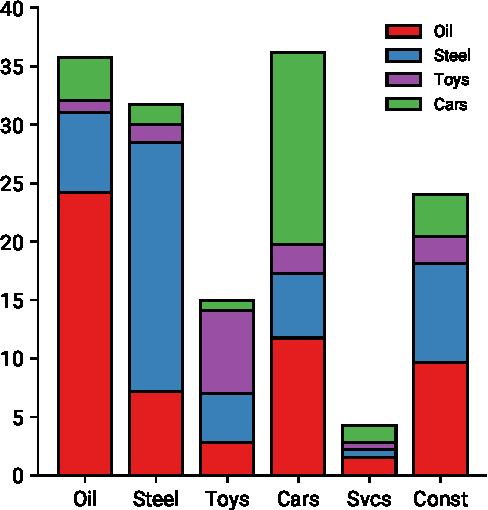
\includegraphics[width=\textwidth]{../programs/python/output/fig_data_linkages_downstream_0.pdf}
        \end{subfigure}
        \hfill
        \begin{subfigure}[t]{0.4\textwidth}
            \centering
            \caption{Intermediate sales (\% GO)}
            \label{fig:us}
            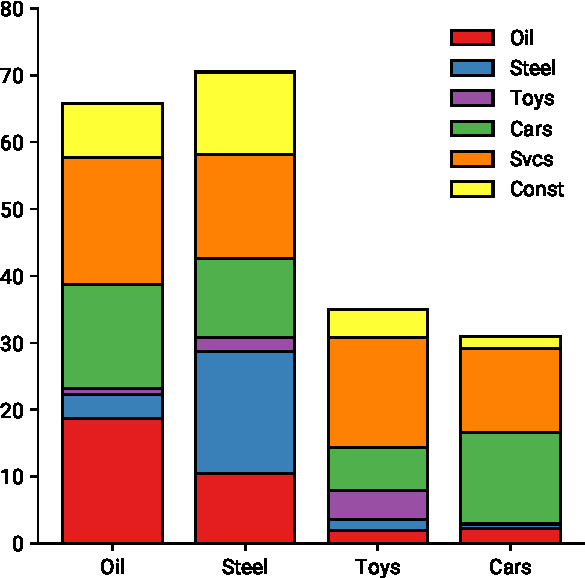
\includegraphics[width=\textwidth]{../programs/python/output/fig_data_linkages_upstream_0.pdf}
        \end{subfigure}
        \hfill
        \begin{subfigure}[t]{0.4\textwidth}
            \centering
            \caption{Imports (\% GO)}
            \label{fig:im1}
            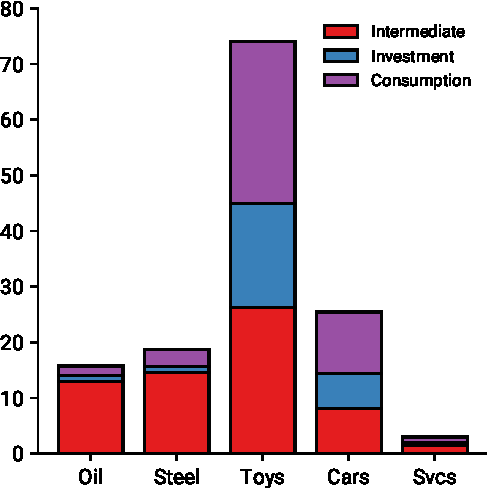
\includegraphics[width=\textwidth]{../programs/python/output/fig_data_sectoral_trade_by_use_im.pdf}
        \end{subfigure}
        \\[2ex]
        \begin{subfigure}[b]{0.4\textwidth}
            \centering
            \caption{Trade balance (\% GO)}
            \label{fig:nx1}
            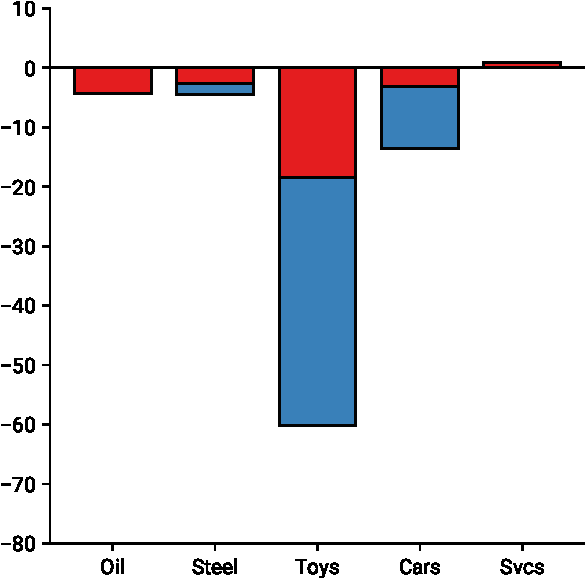
\includegraphics[width=\textwidth]{../programs/python/output/fig_data_sectoral_trade_by_use_nx.pdf}
        \end{subfigure}
        \hfill
        \begin{subfigure}[b]{0.4\textwidth}
            \centering
            \caption{Imports (\% GDP)}
            \label{fig:im2}
            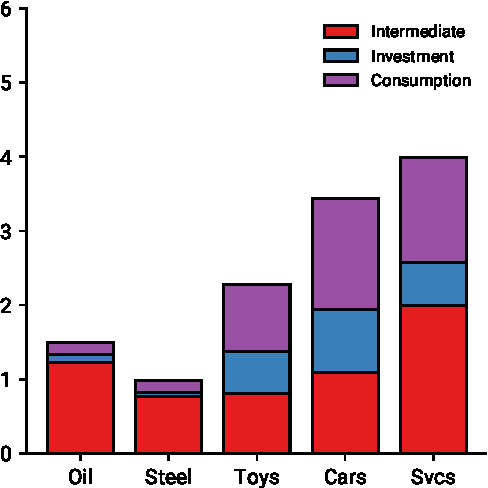
\includegraphics[width=\textwidth]{../programs/python/output/fig_data_sectoral_trade_by_use_im2.pdf}
        \end{subfigure}
        \hfill
        \begin{subfigure}[b]{0.4\textwidth}
            \centering
            \caption{Trade balance (\% GDP)}
            \label{fig:nx2}
            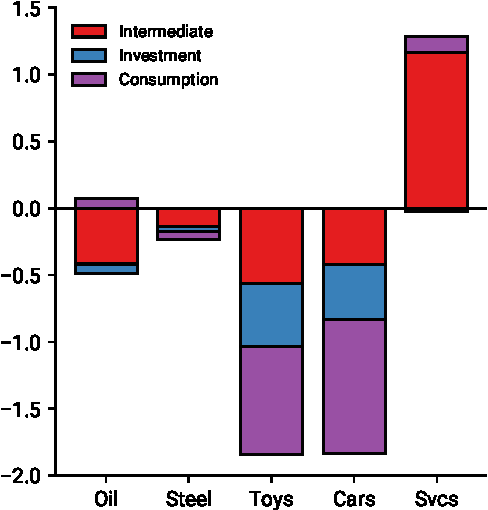
\includegraphics[width=\textwidth]{../programs/python/output/fig_data_sectoral_trade_by_use_nx2.pdf}
        \end{subfigure}
        \begin{fignote}{1.36\textwidth}
            \textit{Notes:} (a) Intermediate input expenditures as percentage of sectoral gross output. (b) Intermediate sales to other sectors as percentage of sectoral gross output. (c) Imports by use (intermediate, consumption, investment) as percentage of sectoral gross output. (d) Same as (c), but net exports instead of imports. (e,f) Same as (c,d) but as percentages of U.S. GDP. Source: 2020 OECD Inter-Country Input-Output Table.
        \end{fignote}
    \end{figure}
\end{landscape}

\begin{landscape}
    \begin{figure}[p]
        \centering
        \caption{Employment effects of U.S. tariffs on goods sectors}
        \label{fig:results1}
        \begin{subfigure}[t]{0.4\textwidth}
            \centering
            \caption{Long-run goods employment}
            \label{fig:lg_lr}
            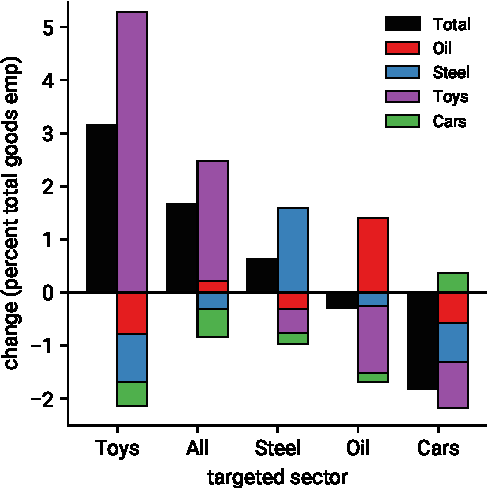
\includegraphics[width=\textwidth]{../programs/python/output/fig_lr_emp_across_scenarios_all_vs_sectors.pdf}
        \end{subfigure}
        \hfill
        \begin{subfigure}[t]{0.4\textwidth}
            \centering
            \caption{Emp. dynamics: tariffs on Toys}
            \label{fig:ls_dyn_s2}
            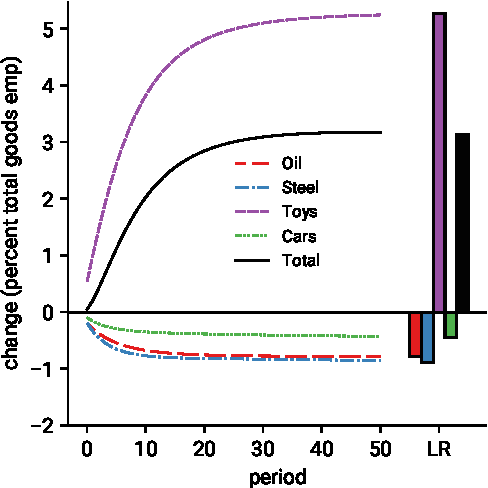
\includegraphics[width=\textwidth]{../programs/python/output/fig_dyn_labor_goods_s2.pdf}
        \end{subfigure}
        \hfill
        \begin{subfigure}[t]{0.4\textwidth}
            \centering
            \caption{Emp. dynamics: tariffs on all goods}
            \ \label{fig:ls_dyn_s4}
            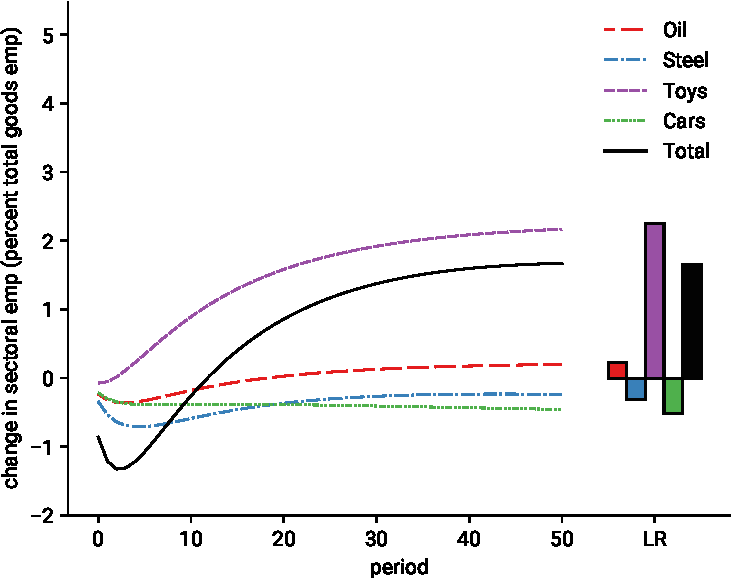
\includegraphics[width=\textwidth]{../programs/python/output/fig_dyn_labor_goods_s4.pdf}
        \end{subfigure}
        \\[2ex]
        \begin{subfigure}[b]{0.4\textwidth}
            \centering
            \caption{Emp. dynamics: tariffs on Steel}
             \label{fig:ls_dyn_s1}
            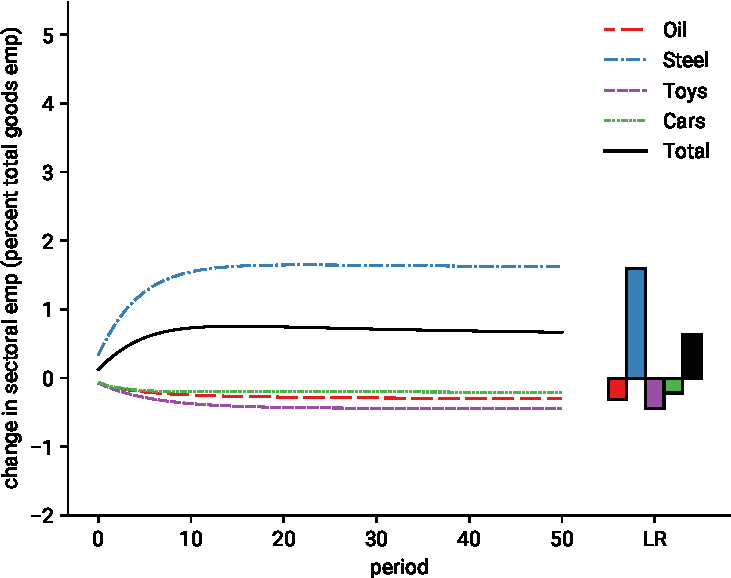
\includegraphics[width=\textwidth]{../programs/python/output/fig_dyn_labor_goods_s1.pdf}
        \end{subfigure}
        \hfill
        \begin{subfigure}[b]{0.4\textwidth}
            \centering
            \caption{Emp. dynamics: tariffs on Oil}
             \label{fig:ls_dyn_s0}
            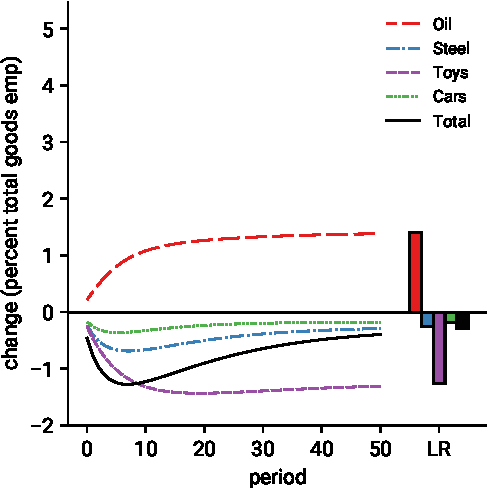
\includegraphics[width=\textwidth]{../programs/python/output/fig_dyn_labor_goods_s0.pdf}
        \end{subfigure}
        \hfill
        \begin{subfigure}[b]{0.4\textwidth}
            \centering
            \caption{Emp. dynamics: tariffs on Cars}
             \label{fig:ls_dyn_s3}
            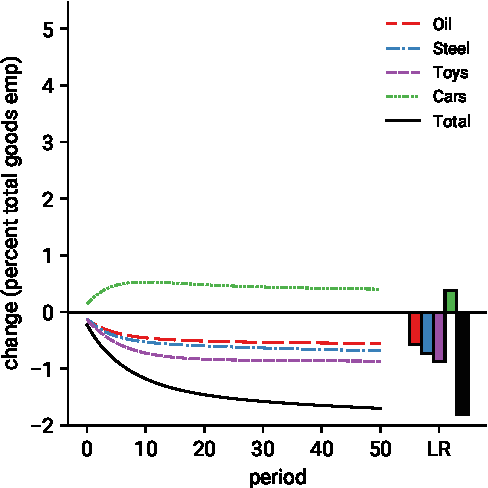
\includegraphics[width=\textwidth]{../programs/python/output/fig_dyn_labor_goods_s3.pdf}
        \end{subfigure}
        \begin{fignote}{1.36\textwidth}
            \textit{Notes:} (a) Long-run change in total employment across all four goods sectors in different tariff scenarios. (b) Sectoral employment dynamics with tariff on high-elasticity downstream goods (``Toys''). (c) Sectoral employment dynamics with tariff on all goods sectors. (d) Sectoral employment dynamics with tariff on low-elasticity upstream goods (``Steel''). (e) Sectoral employment dynamics with tariff on high-elasticity upstream goods (``Oil''). (f) Sectoral employment dynamics with tariff on low-elasticity downstream goods (``Cars'').    
        \end{fignote}
    \end{figure}
\end{landscape}

\begin{landscape}
    \begin{figure}[p]
        \centering
        \caption{Other results and scenarios}
        \label{fig:results2}
        \begin{subfigure}[t]{0.4\textwidth}
            \centering
            \caption{Macroeconomic consequences}
            \label{fig:gdp_lr}
            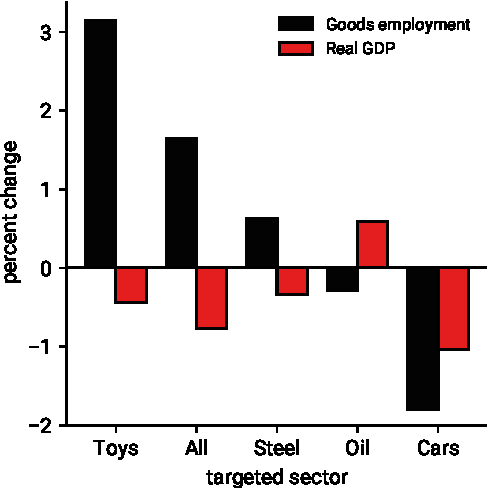
\includegraphics[width=\textwidth]{../programs/python/output/fig_lr_emp_vs_gdp.pdf}
        \end{subfigure}
        \hfill
        \begin{subfigure}[t]{0.4\textwidth}
            \centering
            \caption{Tariffs on one vs. both countries}
            \label{fig:lg_lr_compare}
            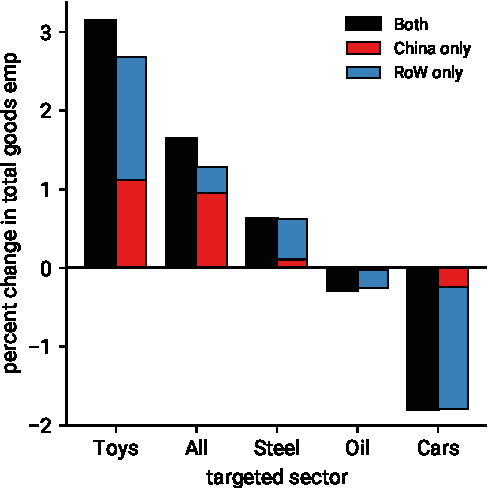
\includegraphics[width=\textwidth]{../programs/python/output/fig_lr_emp_across_scenarios_compare.pdf}
        \end{subfigure}
        \hfill
        \begin{subfigure}[t]{0.4\textwidth}
            \centering
            \caption{Tariffs on only intermediates or final goods}
            \ \label{fig:lg_lr_m_vs_f}
            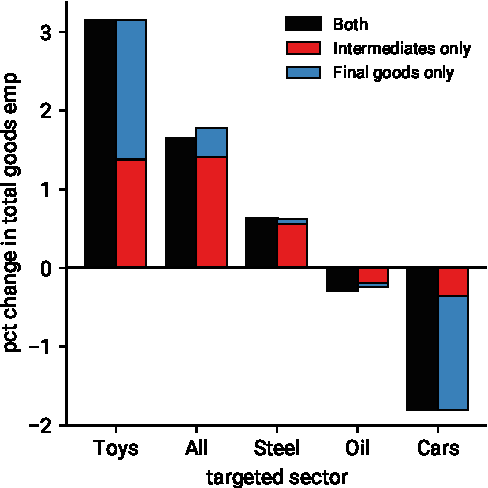
\includegraphics[width=\textwidth]{../programs/python/output/fig_lr_emp_all_vs_m_vs_f.pdf}
        \end{subfigure}
        \\[2ex]
        \begin{subfigure}[b]{0.4\textwidth}
            \centering
            \caption{Tariffs on all goods w/o adj. costs}
             \label{fig:dyn_noadj}
            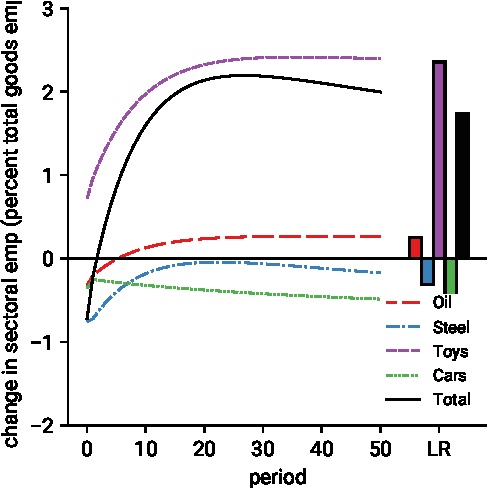
\includegraphics[width=\textwidth]{../programs/python/output/fig_dyn_labor_goods_atb_noadj.pdf}
        \end{subfigure}
        \hfill
        \begin{subfigure}[b]{0.4\textwidth}
            \centering
            \caption{Tariffs on all goods w/ retaliation}
             \label{fig:dyn_retal}
            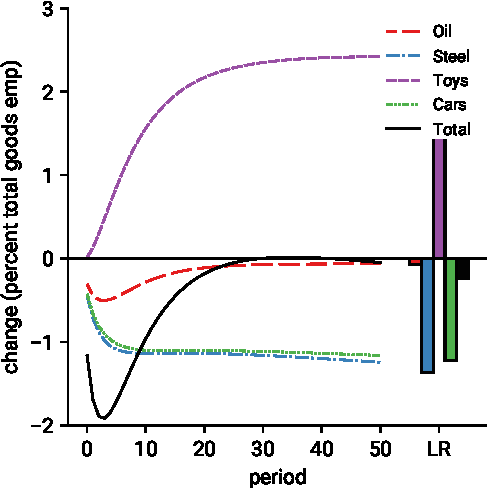
\includegraphics[width=\textwidth]{../programs/python/output/fig_dyn_labor_goods_atb_retaliation.pdf}
        \end{subfigure}
        \hfill
        \begin{subfigure}[b]{0.4\textwidth}
            \centering
            \caption{Temporary tariffs}
             \label{fig:dyn_temp}
            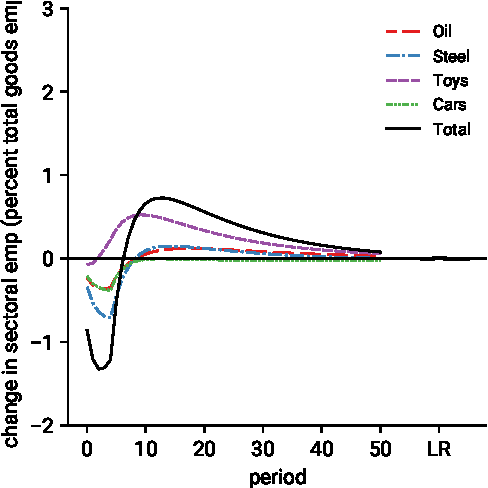
\includegraphics[width=\textwidth]{../programs/python/output/fig_dyn_labor_goods_atb_temp.pdf}
        \end{subfigure}
        \begin{fignote}{1.36\textwidth}
            \textit{Notes:} (a) Long-run effects of tariffs on total goods employment versus real GDP. (b) Long-run employment effects of tariffs on one versus both countries. (c) Long-run effects of tariffs on only intermediate inputs or final goods versus both. (d) Sectoral employment dynamics with tariffs on all goods in model without adjustment frictions. (e) Sectoral employment dynamics with tariffs on all goods and symmetric retaliation by other countries. (f) Sectoral employment dynamics with tariffs on all goods that are unexpectedly reversed after four years.
        \end{fignote}
    \end{figure}
\end{landscape}


\end{document}
